\section{Architecture}
\index{WebRTC}{WebRTC} uses different network techniques to create a connection to a peer. We will explore those techniques and technologies in this chapter.

\subsection{Network Address Translation (\index{NAT}{NAT})}
Is used to give devices in a network a public IP address. This is achieved by translating requests from the device's private IP to the router's public IP with a unique port. The goal is to not need a unique public IP for each device.

\subsection{Session Traversal Utilities for \index{NAT}{NAT} (\index{STUN}{STUN})}
This protocol is used to discover the public address of the peer. It also will determine any restrictions that would prevent a direct connection with a peer.

The peer sends a 'who am i' request to a \index{STUN}{STUN} server which responds with the public address of the peer.

\begin{figure}[H]
	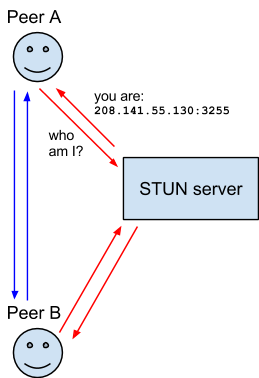
\includegraphics[scale=0.5]{images/webrtc-stun.png}
	\centering
	\caption{\index{STUN}{STUN} communication schema, \url{https://developer.mozilla.org/en-US/docs/Web/API/WebRTC_API/Protocols}}
	\label{fig:STUN}
\end{figure}

There are open \index{STUN}{STUN} servers available (list might not complete):
\begin{itemize}
	\item stun.l.google.com:19302
	\item stun[1-4].l.google.com:19302
	\item stunserver.org
	\item stun.schlund.de
	\item stun.voipstunt.com
\end{itemize}

\subsection{Traversal Using Relays around \index{NAT}{NAT} (\index{TURN}{TURN})}
If \index{STUN}{STUN} can't be used, because for example 'Symmetric \index{NAT}{NAT}' is employed in the network, \index{TURN}{TURN} will be used as fallback. This is achieved by opening a connection with a \index{TURN}{TURN} server, this server then will relaying all information through that server.

\begin{figure}[H]
	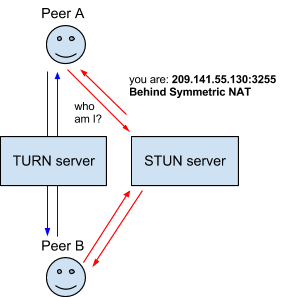
\includegraphics[scale=0.5]{images/webrtc-turn.png}
	\centering
	\caption{\index{TURN}{TURN} communication schema, \url{https://developer.mozilla.org/en-US/docs/Web/API/WebRTC_API/Protocols}}
	\label{fig:TURN}
\end{figure}

There are open \index{TURN}{TURN} servers, for example provided by google. But this will mean all communication is going threw a foreign server which might not be acceptable.

\subsection{Session Description Protocol (SDP)}
This standard describes the multimedia content of a connection. This includes a resolution, formats, codecs, encryption, etc. basically it is the metadata describing the content not the content itself.

\subsection{Interactive Connectivity Establishment (\index{ICE}{ICE}) Candidates}
Peers have to exchange information about the network connection, this is known as an \index{ICE}{ICE} candidate. Each peer proposes its best candidate, and will work down to the worst candidate until they agree on a common candidate.

\subsection{Complete Communication Schema}
The following figure gives an overview over the complete communication mechanism. They also include the fallback mechanisms in case the default is not acceptable.

\begin{figure}[H]
	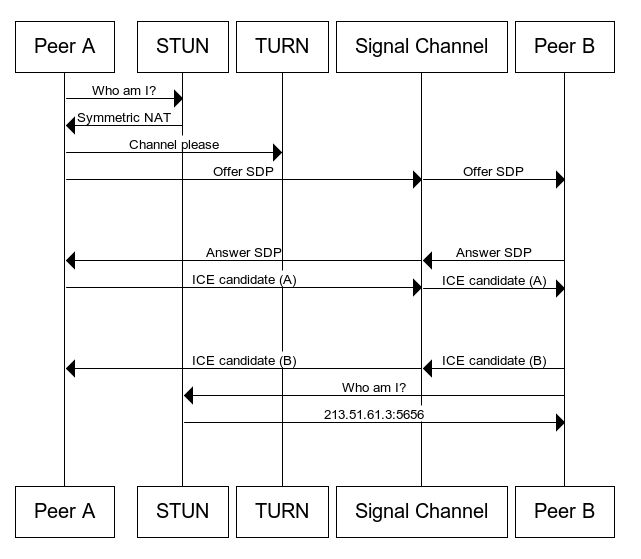
\includegraphics[scale=0.5]{images/webrtc-complete-diagram.png}
	\centering
	\caption{\index{WebRTC}{WebRTC} Complete communication schema, \url{https://developer.mozilla.org/en-US/docs/Web/API/WebRTC_API/Connectivity}}
	\label{fig:WebRTC}
\end{figure}
